\documentclass[journal,twoside,web]{ieeecolor}
\usepackage{jsen,wrapfig}
\usepackage[T1]{fontenc}
\usepackage{amsmath,amssymb,graphicx,booktabs,array,cite}
\usepackage[hidelinks]{hyperref}
\usepackage{url,xurl,balance}
\addtolength{\topmargin}{-5pt}\addtolength{\headheight}{5pt}
\definecolor{abstractbg}{rgb}{0.89804,0.94510,0.83137}
\setlength{\fboxrule}{0pt}\setlength{\fboxsep}{0pt}
\hypersetup{pdftitle={Memory and Time Costs of Drift Compensation and Calibration Transfer for Electronic Noses on Microcontrollers},pdfauthor={Oleksandr Kuznetsov}}
\interdisplaylinepenalty=2500
\setcounter{dbltopnumber}{3}
\renewcommand{\dbltopfraction}{0.88}
\renewcommand{\textfraction}{0.1}
\newcommand{\us}{\ensuremath{\mu\mathrm{s}}}
\hyphenation{micro-controller micro-controllers stan-dard-i-sa-tion}
\begin{document}
\title{Memory and Time Costs of Drift Compensation and Calibration Transfer for Electronic Noses on Microcontrollers}
\author{\mbox{Oleksandr Kuznetsov,~\IEEEmembership{Member,~IEEE}}%
\thanks{O. Kuznetsov is with the Department of Theoretical and Applied Sciences, eCampus University, Italy, and with the Department of Intelligent Software Systems and Technologies, School of Computer Science and Artificial Intelligence, V.N. Karazin Kharkiv National University, Ukraine (e-mail: oleksandr.kuznetsov@uniecampus.it; ORCID: 0000-0003-2331-6326).}\endgraf}
\markboth{IEEE Sensors Journal}{Kuznetsov: Memory and Time Costs of E-Nose Drift Compensation on Microcontrollers}
\IEEEtitleabstractindextext{%
\fcolorbox{abstractbg}{abstractbg}{%
\begin{minipage}{\textwidth}%
\begin{wrapfigure}[17]{r}{3in}%
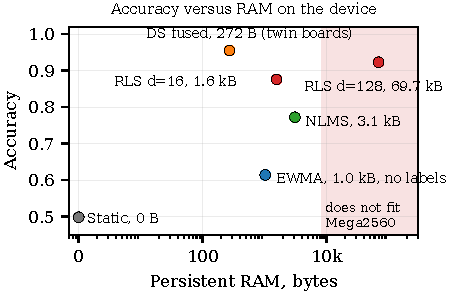
\includegraphics[width=3in]{figures/gagraphic_inline.pdf}%
\end{wrapfigure}%
\begin{abstract}
Like its biological prototype, an electronic nose relies on cross-sensitive receptors whose responses drift over time and differ from one array to another. Compensation methods are usually compared by accuracy alone, although a low-cost instrument has to run them on a microcontroller with a few kilobytes of RAM. In this paper we measure the RAM and the execution time of linear drift-compensation and calibration-transfer methods that adapt a least-squares (ridge) linear classifier, using two public metal-oxide array datasets (36-month drift; five twin boards) and Mega2560, ESP32-C3 and ESP32-S3 boards. Without labels, running standardisation raises the accuracy on the drift stream from 0.498 to 0.614 with 1\,028~B of RAM, in seven of eight test batches. With 20 references per batch drawn from all gases, recursive least squares reaches 0.923 but keeps 69.7~kB in RAM, whereas on 16 compact features it reaches 0.876 with 1.6~kB. A post hoc analysis shows that calibration sessions with a single gas sharply reduce the benefit of label-driven updates and push several of them below the unadapted classifier. Between twin boards, direct standardisation fused into the classifier reaches 0.955 and keeps only 272~B in RAM; its fit and fusion take 0.29~s on the Mega2560. The float32 kernels reproduce the host on complete data streams, both on the host and on the three boards. For slow gas sensing, it is memory rather than time that decides what an 8-bit device can run.
\end{abstract}
\begin{IEEEkeywords}
Calibration transfer, drift compensation, electronic nose, embedded systems, gas sensor arrays, microcontrollers, recursive least squares.
\end{IEEEkeywords}
\end{minipage}}}
\maketitle
\thispagestyle{headings}

\section{Introduction}
\IEEEPARstart{T}{he} electronic nose was proposed as a model of the mammalian olfactory system: instead of one selective receptor per odorant, an array of broadly tuned sensors produces a response pattern, and this pattern is recognised by a trained classifier \cite{persaud}. Metal-oxide (MOX) gas sensors are the most common receptors in such arrays, since they are cheap, sensitive and easy to read out. Their weakness is equally well known. The response of a MOX sensor changes over months because of ageing, poisoning and environmental history, and two nominally identical arrays respond differently to the same gas \cite{marco}. A classifier trained once therefore loses accuracy on the same instrument as time passes, and a classifier trained on one instrument cannot be moved to another without correction.

Both problems have a long history. For long-term drift, component correction \cite{artursson}, orthogonal signal correction \cite{padilla}, common principal components \cite{ziyatdinov}, classifier ensembles \cite{vergara}, domain-adaptation extreme learning machines \cite{zhang} and domain-invariant subspace learning \cite{mida} have been proposed, and a public 36-month dataset \cite{vergara,rodriguez} has become the usual benchmark, although its batches are known to carry temporal confounds \cite{dennler}. Because every labelled sample costs a calibration measurement, later work has reduced the number of labels by active learning on dynamic clusters \cite{liu2019}, by online compensation on large response streams \cite{cao2021} and by cross-domain active learning \cite{sun2022}. For the variation between instruments, direct standardisation (DS), which was developed for spectrometers \cite{wang}, has been applied to twin MOX arrays with only a few transfer samples \cite{fonollosa}. In all these works the methods run on a workstation, and they are judged by accuracy, sometimes together with the number of labels; how much memory and time a method needs on the instrument itself is not reported. A recent review of drift compensation for MOX arrays names the balance between performance and efficiency, and models that can actually be deployed, among the open problems \cite{li2026}. The closest embedded study we are aware of trains a compact neural network for drift compensation offline and quantises it for inference \cite{krayden}; adaptation on the device, its memory and its execution time are not measured there, and we have not found a study that measures them for electronic noses.

For a low-cost electronic nose this gap is important. An Arduino-class 8-bit microcontroller has 8~kB of SRAM, and even ESP32-class devices share a few hundred kilobytes with their communication stacks. A method that updates its model from reference measurements has to keep the model and its own state in RAM between samples, and it may need additional temporary memory when a calibration session ends. Work on learning on the device makes the same point for neural networks, where the memory of the update has to be counted separately from the memory of inference \cite{tinytrain}. On the other hand, the timing requirement of a gas sensor array is mild, because one measurement cycle lasts minutes. It is therefore not obvious in advance whether memory or time limits the choice of method on a given processor.

The aim of this work is to determine, on public recordings of real MOX arrays and on physical microcontrollers, the accuracy, the RAM and the execution time of simple drift-compensation and calibration-transfer methods, and on this basis to show which of them can be deployed on 8-bit and 32-bit devices. We restrict ourselves on purpose to methods that adapt a linear least-squares classifier or a linear feature map. Such methods can be written as short float32 kernels whose memory is known to the byte and which do run on an 8-bit controller with 8~kB of SRAM; ensembles, deep models and kernel methods may be more accurate, but most of them would not fit such a device, and we do not compete with them on accuracy. To achieve this aim, we solve the following tasks, which also form the contribution of the paper.
\begin{enumerate}
\item We compare eight compensation methods and two combinations on the 36-month drift dataset, and eight methods including three calibration-transfer methods on five twin boards, under a protocol whose splits, hyperparameter grids and seeds were fixed before the experiments, and we account for the RAM that each method needs between samples and at the end of a calibration session.
\item We implement the methods that matter for deployment, together with a streaming feature extractor, as float32 C kernels, and we show that they reproduce the host on complete data streams, both in a host replica and on three boards (AVR, RISC-V and Xtensa with a floating-point unit).
\item We measure the time per call on the three boards and examine, in post hoc analyses, how the results change when calibration is less favourable, which leads to a deployment map for 8-bit and 32-bit devices.
\end{enumerate}

\section{Data and Common Model}
\subsection{Datasets}
We use two public datasets of the UCI repository. The first one (D1) is the gas sensor array drift dataset \cite{vergara,rodriguez,uci224}, in its version with concentrations \cite{uci270}. It contains 13\,910 recordings of six gases (ammonia, acetaldehyde, acetone, ethylene, ethanol and toluene) measured by an array of 16 MOX sensors over 36 months and grouped into ten batches. Each recording is described by 128 features, eight per sensor: the steady-state resistance change $\Delta R$, its normalised form, and the maxima and minima of an exponential moving average of the resistance derivative for three smoothing constants, as introduced in \cite{muezzinoglu}. The batches are unbalanced (161 to 3\,613 recordings), and toluene is absent from batches 3--5. Dennler et al.\ have shown that in this dataset the gases were recorded in temporally clustered groups and that the sensor baseline correlates with the recording batch, so that a classifier may exploit drift itself \cite{dennler}. Our evaluation trains only on the first batch and processes the later batches in chronological order, which excludes leakage between training and test batches, but within a batch the arrival of the gases may still be clustered; we therefore also evaluate a stream in which the gases arrive in blocks (Section~\ref{sec:scen}).

The second dataset (D2) contains recordings of five twin arrays of eight Figaro MOX sensors exposed to carbon monoxide, ethanol, ethylene and methane at ten concentration levels \cite{fonollosa,uci361}. Its 640 raw recordings last 600~s at 100~Hz. Each board was measured on different days, boards 1--3 on four days and boards 4 and 5 on two \cite{fonollosa}, but the mapping of the repetition index to the day is not given; we assume that the repetitions follow the order of the days. Fonollosa et al.\ discarded the methane recordings of board 5 because of acquisition problems that corrupted the signals \cite[Sec.~4.3]{fonollosa}, and nine further recordings have missing samples (fewer than 50\,000 of the nominal 60\,000). Our frozen protocol keeps all recordings; the analysis without these recordings is given in Section~\ref{sec:transfer}. All archives were verified by SHA-256 digests before use.

\subsection{Features and classifier}
For D1 we use either all 128 features ($d=128$) or the 16 $\Delta R$ features ($d=16$). For D2 the features are computed by our own streaming extractor (Section~\ref{sec:extractor}), and we use either all eight features of each sensor ($d=64$) or only $\Delta R$ and $\Delta R/R_0$ ($d=16$). Each feature is compressed by the signed logarithm $s(x)=\operatorname{sign}(x)\log(1+|x|)$ and standardised with the mean and standard deviation of the source data, which gives the vector $\boldsymbol z\in\mathbb R^d$.

Except for the adaptive centroids M2, which classify by the nearest class mean, all methods share one linear classifier. With $\boldsymbol a=[\boldsymbol z^T,1]^T$, the predicted class is
\begin{equation}
\hat c=\arg\max_{c}\ \boldsymbol a^T\boldsymbol w_c,\qquad \boldsymbol W=[\boldsymbol w_1,\dots,\boldsymbol w_C]\in\mathbb R^{(d+1)\times C}.
\label{eq:head}
\end{equation}
The head $\boldsymbol W$ is fitted by ridge regression of the $n$ source samples $\boldsymbol A\in\mathbb R^{n\times(d+1)}$ onto one-hot class targets $\boldsymbol T$,
\begin{equation}
\boldsymbol W=(\boldsymbol A^T\boldsymbol A+\boldsymbol\Lambda)^{-1}\boldsymbol A^T\boldsymbol T,\qquad \boldsymbol\Lambda=\operatorname{diag}(\lambda,\dots,\lambda,\epsilon_0),
\label{eq:ridge}
\end{equation}
where the intercept receives only the numerical penalty $\epsilon_0=10^{-9}$; the same convention is used in every ridge fit below. Such a least-squares classifier is weaker than a support-vector machine, but for our purpose it has an important property: the sequential and block estimators described below update exactly the model that is deployed. In float32 the head occupies $4C(d+1)$ bytes, that is, 408~B for $d=16$ and 3\,096~B for $d=128$ in D1 ($C=6$), and 272~B for $d=16$ in D2 ($C=4$). For concentration regression (Section~\ref{sec:e3}), one output per gas predicts $\log_{10}$ of the concentration in ppmv.

\section{Compensation Methods and Memory Accounting}
\label{sec:methods}
We distinguish four kinds of RAM. The \emph{state} of a method is what it keeps between samples in addition to the head, counted in float32 values and one byte per stored class label. The \emph{persistent RAM} adds the head whenever the method modifies it; a method that leaves the head unchanged can keep it in flash memory. \emph{Scratch} memory holds the feature vector of the current sample and the intermediate vectors of one call, and the \emph{calibration peak} is the temporary memory needed when a calibration session ends, for example to solve a least-squares problem. These quantities describe the algorithms; the memory of our test firmware, which keeps every head in RAM for convenience, is reported separately in Section~\ref{sec:memory}.

\emph{M0, static head.} The source model is applied without change and has no state.

\emph{M1, EWMA standardisation.} Without any labels, the running mean $\boldsymbol m$ and variance $\boldsymbol v$ of the incoming features replace the source statistics:
\begin{align}
\boldsymbol m_t&=\boldsymbol m_{t-1}+\alpha(\boldsymbol z_t-\boldsymbol m_{t-1}),\\
\boldsymbol v_t&=(1-\alpha)\bigl(\boldsymbol v_{t-1}+\alpha(\boldsymbol z_t-\boldsymbol m_{t-1})^{\odot 2}\bigr),
\end{align}
and the head receives $(\boldsymbol z_t-\boldsymbol m_t)\oslash(\boldsymbol v_t+\epsilon)^{\odot 1/2}$. The method resembles the adaptation of a receptor to a constant background; its state is $8d+4$~bytes.

\emph{M2--M4, other feature-level corrections.} Adaptive class centroids updated without labels (M2, $4Cd+4$~B), correction along $r$ drift directions estimated from the references in the spirit of component correction \cite{artursson} (M3, $4rd+4$~B), and a per-feature gain and offset fitted to the references (M4, $8d$~B) complete the set. During a calibration session, M4 also accumulates four sums of $d$ values ($16d$~B), which are released after the fit.

\emph{M5, NLMS on the head.} For each reference $(\boldsymbol z,c)$ with one-hot target $\boldsymbol t$, the head is updated as \cite{haykin}
\begin{equation}
\boldsymbol W\leftarrow\boldsymbol W+\frac{\mu}{\|\boldsymbol a\|^2+\epsilon}\,\boldsymbol a\,(\boldsymbol t-\boldsymbol W^T\boldsymbol a)^T .
\end{equation}
Only the step size is stored (4~B), but the head has to be in RAM.

\emph{M6, RLS on the head.} Exponentially weighted RLS keeps the $(d+1)\times(d+1)$ inverse correlation matrix $\boldsymbol P$. We initialise it from the source fit as $\boldsymbol P_0=(\boldsymbol A^T\boldsymbol A+\boldsymbol\Lambda)^{-1}$ with $\boldsymbol\Lambda$ of \eqref{eq:ridge}, so that the first update continues the ridge solution instead of restarting it. With forgetting factor $\beta$,
\begin{align}
\boldsymbol g&=\frac{\boldsymbol P\boldsymbol a}{\beta+\boldsymbol a^T\boldsymbol P\boldsymbol a},\qquad
\boldsymbol W\leftarrow\boldsymbol W+\boldsymbol g(\boldsymbol t-\boldsymbol W^T\boldsymbol a)^T,\\
\boldsymbol P&\leftarrow\beta^{-1}(\boldsymbol P-\boldsymbol g\boldsymbol a^T\boldsymbol P).
\end{align}
The state is $4(d+1)^2+4$~B, i.e., 1\,160~B for $d=16$ but 66\,568~B for $d=128$. Strong forgetting with few informative samples lets $\boldsymbol P$ grow without bound (covariance wind-up); we therefore also examine, post hoc, milder forgetting and a variant in which the trace of $\boldsymbol P$ is bounded by that of $\boldsymbol P_0$ (M6b).

\emph{M7, block least squares.} The $k$ references of one calibration session are buffered, and the head is refitted once by ridge regression shrunk towards the current head,
\begin{equation}
\boldsymbol W\leftarrow\arg\min_{\boldsymbol X}\ \|\boldsymbol T_k-\boldsymbol A_k\boldsymbol X\|_F^2+\operatorname{tr}\bigl((\boldsymbol X-\boldsymbol W)^T\boldsymbol\Lambda_\gamma(\boldsymbol X-\boldsymbol W)\bigr),
\label{eq:block}
\end{equation}
with $\boldsymbol\Lambda_\gamma=\operatorname{diag}(\gamma,\dots,\gamma,\epsilon_0)$. The problem is solved by a Cholesky factorisation of a $(d+1)\times(d+1)$ matrix. The buffer takes $k(4d+1)$~B, and the fit needs the Gram matrix, the solution and the targets as temporary memory.

\emph{M8 and M9, direct standardisation.} For calibration transfer, $k$ pairs of feature vectors of the same gas and concentration, measured on the master and on the slave board, give the affine map $\boldsymbol F\in\mathbb R^{(d+1)\times d}$ from slave to master features, $\boldsymbol z_{\mathrm m}\approx\boldsymbol F^T\boldsymbol a_{\mathrm s}$. We fit it by \eqref{eq:block} with the master features as targets and the prior $[\boldsymbol I,\boldsymbol 0]^T$ in place of $\boldsymbol W$. Stored separately, the map takes $4d(d+1)$~B (1\,088~B for $d=16$). Since the head is linear, the map can be fused into it once after the fit,
\begin{equation}
\boldsymbol W'=\boldsymbol F\,\boldsymbol W_{1:d}+\boldsymbol e_{d+1}\boldsymbol w_{d+1}^T,
\label{eq:fuse}
\end{equation}
where $\boldsymbol W_{1:d}$ are the first $d$ rows of $\boldsymbol W$ and $\boldsymbol w_{d+1}^T$ is its intercept row, so that $\boldsymbol a_{\mathrm s}^T\boldsymbol W'=[\boldsymbol z_{\mathrm m}^T,1]\boldsymbol W$. The fused head occupies $4C(d+1)$~B (272~B for $d=16$) and is applied at the cost of the static head. The per-sensor variant M9 is block diagonal: one affine map of the $q$ features of each sensor ($q=2$ for $d=16$, $q=8$ for $d=64$), fitted in the same way.

Two combinations, M1+M5 and M1+M7, apply the labelled update after the unsupervised standardisation.

\subsection{Streaming feature extractor}
\label{sec:extractor}
The D1 features were computed by the authors of the dataset from complete recordings. For D2 we compute features of the same kind from the raw resistance traces with an extractor that processes one sample at a time and keeps a constant state, as it would on an instrument. During the first 30~s, before the gas reaches the chamber, the extractor accumulates the baseline $R_0$ of each sensor; afterwards it tracks the minimum resistance $R_{\min}$. For each of three smoothing constants $\alpha\in\{0.001,0.01,0.1\}$ it updates an exponential moving average of the first difference of the resistance and keeps its maximum and minimum. At the end of a recording, the eight features of each sensor are $\Delta R=R_0-R_{\min}$, $\Delta R/R_0$ and the six extrema. For eight sensors the state takes 426~B on the Mega2560 and 428~B on the ESP32 boards, which differ only in structure padding.

\section{Protocol}
\label{sec:protocol}
The protocol of E1--E5, with its data splits, hyperparameter grids, selection rules and random seeds, was written down and committed to the public repository before each experiment was run (E1/E2 and E3/E4 separately), and the results were not used to change it. Hyperparameters were selected only on D1 batch 2 and on the D2 board pair $1\rightarrow2$, which are excluded from all reported averages. The analyses E6 and E7 were added after an internal review of the first draft. They change no frozen setting, are reported as post hoc, and are logged with their reasons in the repository.

\emph{E1, static settings.} The head is trained on batch 1 and tested on batches 2--10 (setting 1), or trained on batch $b-1$ and tested on batch $b$ (setting 2); a multinomial logistic head is included for reference.

\emph{E2, streaming drift compensation (main experiment).} Batches 2--10 of D1 are processed in order, and the state of every method carries over from batch to batch. In each batch a seeded permutation fixes the order of the samples; the first $k\in\{0,1,5,20\}$ samples are labelled references, i.e., one calibration session, and the remaining samples are classified in order without labels. The references are thus drawn uniformly from all gases present in the batch, which is a favourable condition. Accuracy and macro-F1 are averaged over batches 3--10 and 20 permutation seeds. The ridge parameter of the head and the hyperparameters of the methods were selected from fixed grids by the mean accuracy on batch 2, with five separate tuning seeds and $k=5$.

\emph{E3, concentration under drift.} \label{sec:e3} The gas identity is assumed to be known, and one regression head per gas predicts $\log_{10}$ ppmv. The stream contains only the recordings of that gas, so that $k$ references per batch are $k$ references of that gas. Budgets and selection otherwise follow E2, and the metric is the root-mean-square error (RMSE) averaged over gases.

\emph{E4, calibration transfer and day-to-day drift.} The head is trained on all recordings of a master board and applied to a slave board, for all 20 ordered pairs. For $k\in\{0,2,4,8,16,40\}$, $k$ of the 40 gas--level conditions are drawn at random per seed, and their first-day recordings on both boards form transfer pairs (M4, M8, M9) or labelled references (M5--M7). All other recordings of the slave board are evaluated; M1 uses no labels, and its results at $k>0$ are computed on the same evaluation records as those of the other methods. We report the mean and the worst of the 19 pairs other than the tuning pair, over 20 seeds. Within boards 1--3, we also train on the first day and test on the following ones.

\emph{E5, microcontrollers.} The kernels of Section~\ref{sec:methods} and the feature extractor were written in C and compiled with \texttt{-fno-fast-math -ffp-contract=off} both for the host and for the boards. A fixture of real samples is stored in flash: 64 and 32 recordings of D1 batch 7 for $d=16$ and $d=128$ with the frozen E2 heads and hyperparameters, 20 references and 44 test recordings for the block refit, 16 transfer pairs and 64 test recordings from D2 boards $1\rightarrow2$ for DS, and 512 samples of one raw D2 recording for the extractor. Each kernel first runs once and is checked against the host reference output; only a kernel that passes is timed ten times with \texttt{micros()}. Each board was flashed once and measured in two sessions. Table~\ref{tab:boards} lists the boards and builds.

\emph{E6, post hoc host analyses.} (i) All E2 streams of M0, M1, M5--M7 and the two combinations, and the E4 runs of DS at $k=8$ and 16 for $d=16$ and 64, were repeated with the float32 C kernels of the firmware and compared prediction by prediction with the float64 host; for DS the fused head \eqref{eq:fuse} was compared as well. The extractor was run over all 640 complete D2 recordings. (ii) E2 was repeated with the recordings of each batch arriving in blocks of one gas, and with all $k$ references of a session drawn from one gas; E4 was repeated with the 16 transfer pairs drawn from the four lowest concentration levels, from two gases or from one gas. (iii) Implementation variants: block least squares with the intercept penalised like the weights (M7b), RLS with bounded trace (M6b), and RLS with forgetting factors 0.95 and 0.99 in E2 and E3. (iv) E4 without the methane recordings of board 5 and without the nine recordings with missing samples, and a matrix of training and test days within each board.

\emph{E7, complete streams on the boards.} A second firmware receives real samples over USB. It runs the complete E2 stream of seed 0 with $k=20$ for M0, M1, M5, M6, M7 and M1+M5 at $d=16$ on all boards, and for M0, M1, M5, M6 and M1+M5 at $d=128$ on the ESP32 boards; it fits DS on the board for three board pairs and fuses it into the head, and it passes complete 600~s D2 recordings through the extractor. The peak stack depth is recorded by stack painting on the Mega2560 and by the high-water mark of the loop task on the ESP32 boards.

\emph{Statistics.} The eight test batches of E2 form one stream whose state carries over, and the 19 board pairs of E4 share boards and recordings, so neither can be treated as independent units. For E2 we therefore report the differences per batch (mean, number of batches in favour and range); intervals over the 20 reference draws are narrow and describe only this one stream. For E4 we use a cluster bootstrap that resamples the five boards with replacement and averages the differences over all ordered pairs of distinct drawn boards (10\,000 replicates) \cite{davison}. With five clusters such intervals are coarse, and we read them as an indication of direction rather than as strong evidence. Both methods of every comparison are evaluated on identical test records.

\begin{table}[t]
\caption{Boards, Toolchains and Firmware Size (E5)}
\label{tab:boards}\centering\scriptsize\setlength{\tabcolsep}{2.5pt}
\begin{tabular}{l l r r r}\toprule
Board & Core, clock & FPU & RAM used (B) & Flash used (B)\\\midrule
Mega2560 & AVR, 16 MHz & no & 5\,497 / 8\,192 & 67\,378\\
ESP32-C3 & RV32IMC, 160 MHz & no & 84\,812 / 327\,680 & 348\,758\\
ESP32-S3 & Xtensa LX7, 240 MHz & single & 89\,412 / 327\,680 & 362\,101\\\bottomrule
\multicolumn{5}{p{0.9\columnwidth}}{\scriptsize Arduino framework via PlatformIO; avr-gcc 7.3.0 for Mega2560, GCC 8.4.0 (esp-2021r2-patch5) for the ESP32 boards, default \texttt{-Os}. RAM includes a static arena of 4\,600 B on Mega2560 and 70\,724 B on the ESP32 boards.}
\end{tabular}
\end{table}

\section{Results on the Host}
\subsection{Drift over 36 months}
In the static settings of E1, a head trained on batch 1 reaches only 0.542 on batches 2--10 with all 128 features and 0.468 with 16 features, whereas retraining on the previous batch gives 0.783 and 0.606. Retraining, however, needs the labels of a whole batch and either the batch itself (up to 3\,613 recordings, about 1.9~MB at $d=128$) or its normal equations ($4(d+1)(d+1+C)$~B, i.e., 69.7~kB at $d=128$ and 1.6~kB at $d=16$), so we use it only as a frame for the streaming results.

\begin{table*}[!t]
\caption{Drift Compensation on the Gas Sensor Array Drift Data: Accuracy (Batches 3--10, 20 Seeds) and Persistent State}
\label{tab:e2}\centering\footnotesize
\begin{tabular}{l rrrr r @{\hspace{14pt}} rrrr r}\toprule
 & \multicolumn{5}{c}{$d=16$} & \multicolumn{5}{c}{$d=128$}\\\cmidrule(lr){2-6}\cmidrule(lr){7-11}
Method & $k=0$ & 1 & 5 & 20 & State (B) & $k=0$ & 1 & 5 & 20 & State (B)\\\midrule
Static head & 0.434 & 0.434 & 0.434 & 0.433 & 0 & 0.498 & 0.498 & 0.498 & 0.498 & 0\\
EWMA standardisation & 0.541 & 0.541 & 0.541 & 0.541 & 132 & 0.614 & 0.614 & 0.614 & 0.614 & 1\,028\\
NLMS on head & -- & 0.447 & 0.479 & 0.574 & 4 & -- & 0.579 & 0.676 & 0.772 & 4\\
RLS on head & -- & 0.447 & 0.631 & 0.876 & 1\,160 & -- & 0.634 & 0.792 & 0.923 & 66\,568\\
Block OLS on head & -- & 0.243 & 0.614 & 0.898 & 1\,300 & -- & 0.481 & 0.721 & 0.855 & 10\,260\\
EWMA + NLMS & -- & 0.546 & 0.557 & 0.575 & 136 & -- & 0.645 & 0.710 & 0.798 & 1\,032\\
EWMA + block OLS & -- & 0.246 & 0.591 & 0.842 & 1\,432 & -- & 0.503 & 0.671 & 0.803 & 11\,288\\
\bottomrule\end{tabular}
\end{table*}


Table~\ref{tab:e2} and Fig.~\ref{fig:frontier}(a) summarise E2, and Table~\ref{tab:stats} gives the paired differences. Without any labels, EWMA standardisation improves the static head from 0.434 to 0.541 at $d=16$ (132~B) and from 0.498 to 0.614 at $d=128$ (1\,028~B), and the macro-F1 from 0.346 to 0.435 and from 0.387 to 0.560. The gain is not uniform: it is positive in six and seven of the eight test batches, while in the remaining batches EWMA loses up to 0.095. Adaptive centroids lower the accuracy (0.302 and 0.436), and the per-feature affine correction stays near the static head (0.465 and 0.464 at $k=20$). Component correction, on the other hand, profits from the references at $d=128$ and reaches 0.658 at $k=20$ with 1\,540~B, which is more than EWMA; at $d=16$ it reaches 0.503.

\begin{table}[t]
\caption{Paired Differences in Accuracy}
\label{tab:stats}\centering\scriptsize\setlength{\tabcolsep}{2pt}
\begin{tabular}{l r r l}\toprule
Comparison & Mean & Better & 95\% interval\\\midrule
\multicolumn{4}{l}{\emph{E2, drift stream: units are the 8 test batches}}\\
M1 vs M0, $d=16$, $k=0$ & +0.107 & 6/8 & [-0.09, +0.38]$^a$\\
M1 vs M0, $d=128$, $k=0$ & +0.116 & 7/8 & [-0.09, +0.26]$^a$\\
M5 vs M0, $d=128$, $k=20$ & +0.274 & 8/8 & [+0.17, +0.51]$^a$\\
M6 vs M5, $d=128$, $k=20$ & +0.151 & 8/8 & [+0.05, +0.29]$^a$\\
M7 vs M6, $d=16$, $k=20$ & +0.022 & 4/8 & [-0.05, +0.16]$^a$\\
M6 vs M5, $d=16$, $k=20$ & +0.302 & 8/8 & [+0.12, +0.47]$^a$\\
\multicolumn{4}{l}{\emph{E4, transfer: units are the 19 board pairs}}\\
M1 $k=0$ vs M0 $k=0$ & +0.065 & 15/19 & [+0.008, +0.138]$^b$\\
M8 $k=16$ vs M1 $k=16$ & +0.049 & 16/19 & [-0.004, +0.123]$^b$\\
M8 $k=16$ vs M6 $k=16$ & +0.022 & 13/19 & [+0.003, +0.045]$^b$\\
M8 $d=16$ vs $d=64$, $k=16$ & +0.009 & 10/19 & [-0.013, +0.040]$^b$\\
M1 $k=16$ vs M1 $k=0$ & +0.011 & 15/19 & [-0.000, +0.020]$^b$\\
M8 $k=8$ vs M1 $k=8$ & +0.025 & 11/19 & [-0.006, +0.071]$^b$\\
\bottomrule
\multicolumn{4}{p{0.95\columnwidth}}{\scriptsize $^a$Range of the per-batch differences; an interval over the 20 reference draws would only describe this one stream and is given in the repository. $^b$Percentile interval of a cluster bootstrap that resamples the five boards (10\,000 replicates). Both comparisons in a row use identical test records.}
\end{tabular}
\end{table}


Labels change the picture more strongly. With 20 references per batch, NLMS at $d=128$ reaches 0.772 and is better than the static head in all eight batches; it keeps only 4~B of state, but the modified head adds 3\,096~B. RLS gives the highest accuracy, 0.923, and exceeds NLMS in every batch, but together with the head its covariance matrix keeps 69.7~kB in RAM, more than eight times the SRAM of the Mega2560. On the 16 compact features the same RLS keeps 1.6~kB and reaches 0.876, and block least squares reaches 0.898 with 1.7~kB and a 3.8~kB peak at the refit. The two are close: block least squares is better in four of the eight batches, by 0.022 on average.

One reference per batch is not enough, and block least squares even collapses to 0.243 at $d=16$. Two causes contribute to this. Its shrinkage $\gamma=0.1$ was selected at $k=5$, and with a single one-hot target the almost unpenalised intercept moves freely towards that class. When the intercept is penalised like the weights (M7b, post hoc), the result rises to 0.313 at $d=16$ and from 0.481 to 0.590 at $d=128$, which is still below the static head at $d=16$; at $k\ge5$ the variant changes the result by at most 0.011.

\begin{figure*}[!t]
\centering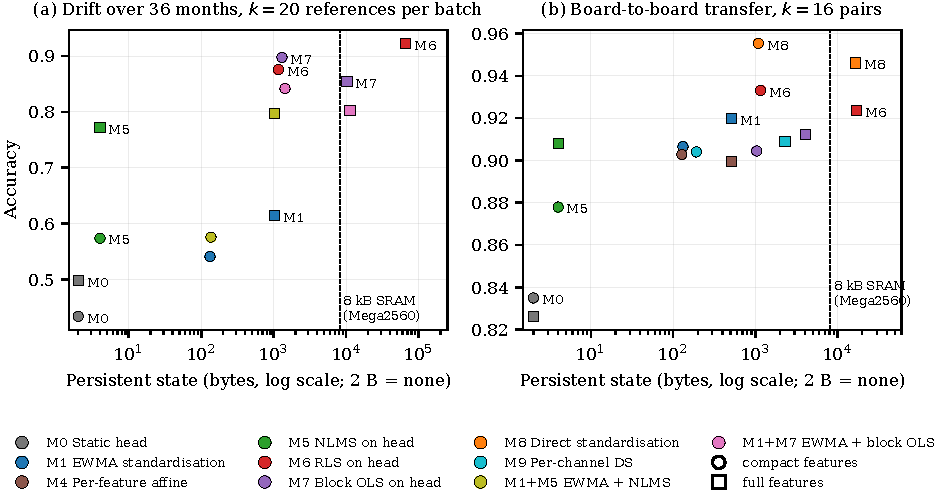
\includegraphics[width=\textwidth]{figures/frontier.pdf}
\caption{Accuracy versus persistent RAM (adaptation state plus the head if the method modifies it; DS fused into the head). (a) D1 drift stream, batches 3--10, $k=20$ references per batch. (b) D2 transfer, mean over 19 board pairs, $k=16$ transfer pairs or references. Circles: compact features ($d=16$); squares: full features ($d=128$ in D1, $d=64$ in D2). The static head needs no RAM beyond the feature vector and is drawn at 0. Points to the right of the dashed line (8~kB SRAM of the Mega2560, which must also hold the stack and the application) do not fit that board.}
\label{fig:frontier}
\end{figure*}

\subsection{Less favourable calibration (post hoc)}
\label{sec:scen}
\begin{table}[t]
\caption{Drift Stream Under Less Favourable Calibration ($k=20$, Accuracy, Batches 3--10)}
\label{tab:scen}\centering\scriptsize\setlength{\tabcolsep}{3pt}
\begin{tabular}{l r rrrr}\toprule
 & & \multicolumn{2}{c}{References of all gases} & \multicolumn{2}{c}{References of one gas}\\\cmidrule(lr){3-4}\cmidrule(lr){5-6}
Method & $d$ & shuffled & gas blocks & shuffled & gas blocks\\\midrule
M1 EWMA & 16 & 0.541 & 0.514 & 0.544 & 0.520\\
M5 NLMS & 16 & 0.574 & 0.565 & 0.391 & 0.371\\
M6 RLS & 16 & 0.876 & 0.867 & 0.329 & 0.313\\
M7 block OLS & 16 & 0.898 & 0.890 & 0.136 & 0.134\\
M1+M5 EWMA + NLMS & 16 & 0.575 & 0.554 & 0.424 & 0.396\\
\midrule
M1 EWMA & 128 & 0.614 & 0.541 & 0.615 & 0.538\\
M5 NLMS & 128 & 0.772 & 0.752 & 0.472 & 0.462\\
M6 RLS & 128 & 0.923 & 0.924 & 0.536 & 0.522\\
M7 block OLS & 128 & 0.855 & 0.855 & 0.355 & 0.366\\
M1+M5 EWMA + NLMS & 128 & 0.798 & 0.675 & 0.597 & 0.485\\
\bottomrule
\multicolumn{6}{p{0.95\columnwidth}}{\scriptsize First column: protocol of E2. Gas blocks: within each batch the recordings arrive grouped by gas in a random gas order. One gas: all $k$ references of a session come from one randomly chosen gas. 20 seeds; the 95\% intervals over seeds are at most $\pm0.036$ and are given in the repository.}
\end{tabular}
\end{table}

The references of E2 come from all gases of a batch, and the recordings arrive in random order. Table~\ref{tab:scen} relaxes both conditions. When the recordings of a batch arrive in blocks of one gas, EWMA standardisation suffers most, because its running statistics follow the current gas: at $d=128$ its accuracy falls from 0.614 to 0.541. The label-driven methods are almost insensitive to the order, since their references still cover all gases. When, however, all references of a session come from one gas, as in a calibration with a single test gas, the benefit of the references largely disappears. At $d=16$ every label-driven update falls below the static head of 0.435; block least squares falls to 0.136, because the refit pulls the head towards the one class it sees. At $d=128$, NLMS (0.472) and block least squares (0.355) fall below the static head of 0.500, whereas RLS (0.536) and EWMA+NLMS (0.597) stay above it but lose 0.39 and 0.20 compared with references from all gases. Labelled adaptation of the classifier therefore requires calibration sessions that cover the classes, and in practice this requirement matters more than the choice between NLMS, RLS and block least squares. Where a session can contain only one gas, a field protocol should either collect the references of several sessions before an update or restrict the update to the feature level, as EWMA does.

\subsection{Implementation variants (post hoc)}
The selected RLS forgetting factor $\beta=0.9$ lies on the edge of the E2 grid. With $\beta=0.95$, the accuracy at $d=128$ and $k=20$ rises from 0.923 to 0.940, whereas at $d=16$ it falls from 0.876 to 0.813; $\beta=0.99$ gives 0.909 and 0.654. Bounding the trace of $\boldsymbol P$ (M6b) prevents wind-up but lowers the accuracy at $d=16$, $k=20$ to 0.613, because the update then follows the drift too slowly. The edge selection therefore did not hide a large gain, and we keep the frozen values; the reported RLS figures nevertheless depend on $\beta$ by several points, and an adaptive forgetting factor would be a natural refinement.

\subsection{Concentration under drift}
\begin{table}[t]
\caption{Concentration Regression Under Drift: RMSE in $\log_{10}$ ppmv (Batches 3--10, Six Gases, 20 Seeds)}
\label{tab:e3}\centering\footnotesize\setlength{\tabcolsep}{3.5pt}
\begin{tabular}{l rrr rrr}\toprule
 & \multicolumn{3}{c}{$d=16$} & \multicolumn{3}{c}{$d=128$}\\\cmidrule(lr){2-4}\cmidrule(lr){5-7}
Method & $k=1$ & 5 & 20 & $k=1$ & 5 & 20\\\midrule
Static head & 0.312 & 0.312 & 0.329 & 0.326 & 0.326 & 0.340\\
EWMA standardisation & 0.352 & 0.353 & 0.364 & 0.241 & 0.241 & 0.249\\
NLMS on head & 0.308 & 0.294 & 0.274 & 0.183 & 0.154 & 0.140\\
RLS on head & 0.283 & 0.193 & 0.322$^\dagger$ & 0.182 & 0.148 & 0.317$^\dagger$\\
Block OLS on head & 0.224 & 0.184 & 0.174 & 0.176 & 0.138 & 0.119\\
\bottomrule
\multicolumn{7}{p{0.95\columnwidth}}{\scriptsize Gas identity known; $k$ references of that gas per batch. $^\dagger$RLS with the selected $\beta=0.8$ winds up at $k=20$ for toluene and ammonia (worst gas 0.95 at $d=16$); with $\beta=0.95$ (post hoc) it gives 0.171 and 0.124.}
\end{tabular}
\end{table}

For regression (Table~\ref{tab:e3}), the static heads have an RMSE of 0.31--0.34 in $\log_{10}$ ppmv, i.e., a typical error of a factor of about two in concentration. Without labels, EWMA standardisation helps at $d=128$ (0.241) but hurts at $d=16$ (0.352): within one gas the incoming mixture of concentrations differs from that of the source, and standardisation removes part of the concentration signal itself. With five references of the gas, NLMS at $d=128$ reduces the RMSE to 0.154 with 4~B of state, and block least squares to 0.138. RLS with the selected forgetting factor $\beta=0.8$, again on the edge of the grid, becomes unstable for toluene and ammonia at $k=20$ (worst gas 0.95 at $d=16$), which is the covariance wind-up described in Section~\ref{sec:methods}. With $\beta=0.95$ (post hoc), RLS is stable and reaches 0.171 at $d=16$ and 0.124 at $d=128$, with a worst gas of 0.27 and 0.19.

\subsection{Calibration transfer between twin boards}
\label{sec:transfer}
\begin{table}[t]
\caption{Calibration Transfer Between Twin Boards: Mean (Worst) Accuracy Over 19 Board Pairs, $d=16$}
\label{tab:e4}\centering\scriptsize\setlength{\tabcolsep}{2pt}
\begin{tabular}{l rrrr r}\toprule
Method & $k=0$ & 4 & 8 & 16 & State (B)\\\midrule
M0 static & 0.831 (0.65) & 0.831 (0.66) & 0.832 (0.67) & 0.835 (0.70) & 0\\
M1 EWMA & 0.895 (0.71) & 0.899 (0.70) & 0.900 (0.71) & 0.907 (0.71) & 132\\
M4 affine & -- & 0.889 (0.74) & 0.896 (0.73) & 0.903 (0.73) & 128\\
M9 chan. DS & -- & 0.891 (0.74) & 0.898 (0.74) & 0.904 (0.74) & 192\\
M8 DS & -- & 0.878 (0.75) & 0.925 (0.87) & 0.955 (0.92) & 1\,088\\
M5 NLMS & -- & 0.845 (0.72) & 0.855 (0.72) & 0.878 (0.72) & 4\\
M6 RLS & -- & 0.878 (0.72) & 0.902 (0.74) & 0.933 (0.85) & 1\,160\\
M7 block OLS & -- & 0.848 (0.70) & 0.876 (0.74) & 0.904 (0.79) & 1\,040\\
\midrule
M8 DS, $d=64$ & -- & 0.890 (0.75) & 0.919 (0.77) & 0.946 (0.87) & 16\,640\\
\bottomrule\end{tabular}
\end{table}

Board-to-board variation is the more severe problem in D2 (Table~\ref{tab:e4}, Fig.~\ref{fig:frontier}(b)). A master head applied to a slave board reaches 0.831 on average, with a worst pair of 0.65. Within a board, by contrast, a head trained on any one day and tested on any other day of the same board reaches 0.875--1.000 at $d=16$ (post hoc, all orders of the days), so that the day-to-day drift in D2 is mild whatever the order of the repetitions. EWMA standardisation of the slave stream, again without labels, raises the transfer accuracy to 0.895 with 132~B; the gain of 0.065 has a board-bootstrap interval of $[0.008, 0.138]$. DS on the compact features reaches 0.925 with eight transfer pairs and 0.955 with sixteen, with a worst pair of 0.92, and since it can be fused into the head, only 272~B remain in RAM. Compared with EWMA on the same records, DS is better in 16 of 19 pairs by 0.049, but with five boards the interval $[-0.004, 0.123]$ includes zero. Compared with RLS on the head it is better by 0.022, with an interval of $[0.003, 0.045]$, which we read as a likely direction rather than a firm result. DS on all 64 features is not better (0.946), and the paired affine and per-sensor corrections stay at 0.89--0.90, at the level of EWMA, which needs no transfer samples at all.

Without the corrupted methane recordings of board 5, a head trained on board 5 cannot recognise methane, so we compare the 15 pairs whose master is another board. On these pairs DS reaches 0.954 (0.957 with all recordings), RLS 0.951, the affine and per-sensor corrections 0.947, EWMA 0.940 at $k=16$ and 0.926 without labels, and the static head 0.857. The cleaned data thus confirm the gain of all transfer methods over the static head but shrink the differences between them to less than 0.015; for practical conclusions we rely on these cleaned figures. Removing the nine recordings with missing samples changes no mean by more than 0.003.

\begin{table}[t]
\caption{Transfer With Transfer Pairs From Restricted Conditions ($d=16$, $k=16$, Post Hoc)}
\label{tab:conc}\centering\scriptsize\setlength{\tabcolsep}{2.2pt}
\begin{tabular}{l rrrrrrr}\toprule
Pairs drawn from & M0 & M1 & M4 & M9 & M8 & M6 & M7\\\midrule
16 of 40 conditions (E4) & 0.835 & 0.907 & 0.903 & 0.904 & 0.955 & 0.933 & 0.904\\
4 lowest levels, all gases & 0.833 & 0.912 & 0.903 & 0.904 & 0.967 & 0.936 & 0.919\\
Two gases, all levels & 0.831 & 0.901 & 0.876 & 0.869 & 0.825 & 0.836 & 0.773\\
One gas (10 pairs) & 0.830 & 0.899 & 0.847 & 0.844 & 0.785 & 0.804 & 0.734\\
\bottomrule
\multicolumn{8}{p{0.95\columnwidth}}{\scriptsize Mean accuracy over 19 board pairs and 20 seeds; the gases are drawn per seed. M0 and M1 do not use the pairs and change only because the evaluated records differ slightly.}
\end{tabular}
\end{table}


The transfer pairs of E4 are drawn from all 40 gas--level conditions. Table~\ref{tab:conc} shows that the choice of these conditions matters as much for DS as for the classifier updates of D1. Pairs from the four lowest concentration levels of all gases work as well as random pairs (0.967), but pairs from only two gases bring DS down to 0.825, close to the static head, and pairs from one gas to 0.785, below it; RLS and block least squares behave in the same way. EWMA, which uses no pairs, keeps 0.90 in all cases. A transfer session should therefore include every gas of interest, even at low concentrations, and when this is impossible, unsupervised standardisation is the safer choice.

\section{Execution on Microcontrollers}
\subsection{Agreement with the host}
All six E5 sessions (two per board) passed validation: each kernel reproduced the host predictions on every fixture sample, the checksums of the updated heads and of the DS map differed from the host by at most $3\times10^{-6}$ relative, and the extractor reproduced the host features exactly. RLS at $d=128$ does not fit the Mega2560 and is reported there as skipped.

Because the fixtures are short, E6 repeated the complete streams with the same float32 C kernels on the host. Over 920 complete E2 streams, 65 of 12.3 million predictions differ from the float64 host, and no accuracy changes by more than $1.3\times10^{-5}$; the differences occur where two class scores are nearly equal, mostly in RLS. DS fitted in float32 and fused into the head agrees with the separate float64 map on all 86\,880 predictions at $d=16$ and on all but 2 of 86\,880 at $d=64$. The extractor gives bit-identical features on all 640 complete recordings (38.0 million samples).

On the boards themselves (E7, Table~\ref{tab:e7}), the configurations listed in Section~\ref{sec:protocol} were run over complete streams of 13\,285 predictions each: six on the Mega2560 and eleven on each ESP32. All methods except RLS reproduced the host float32 predictions without exception. RLS differed in 1 of 13\,285 predictions on the Mega2560, and in 2 at $d=16$ and 4 at $d=128$ on the ESP32 boards, again where two class scores nearly coincide, since the target libraries round some float32 operations differently from the host. DS was fitted on the board from 16 transfer pairs and fused into the head, and the resulting accuracy on pairs $1\rightarrow3$, $1\rightarrow4$ and $1\rightarrow5$ equalled the host value on every board. Fed with three complete 600~s recordings (173\,000 samples), the extractor returned features within $1.5\times10^{-8}$ relative of the host; this small difference comes from the decimal transfer of the result. M2--M4, M9, M1+M7 and block least squares at $d=128$ were not run on the boards; their kernels consist of the same operations as those tested.

\begin{table}[t]
\caption{RAM of the Firmware Configurations in Bytes (float32)}
\label{tab:ram}\centering\scriptsize\setlength{\tabcolsep}{2pt}
\begin{tabular}{l r r r r r r r}\toprule
Configuration & $d$ & Head & State & Persist. & Scratch & Calib. & Peak\\\midrule
M0 Static head & 16 & -- & -- & 0 & 64 & -- & 64\\
M1 EWMA & 16 & -- & 132 & 132 & 64 & -- & 196\\
M5 NLMS & 16 & 408 & 4 & 412 & 64 & -- & 476\\
M6 RLS & 16 & 408 & 1\,160 & 1\,568 & 132 & -- & 1\,700\\
M7 Block OLS & 16 & 408 & 1\,300 & 1\,708 & 64 & 2\,044 & 3\,816\\
M1+M5 EWMA + NLMS & 16 & 408 & 136 & 544 & 64 & -- & 608\\
M1+M7 EWMA + OLS & 16 & 408 & 1\,432 & 1\,840 & 64 & 2\,044 & 3\,948\\
M0 Static head & 128 & -- & -- & 0 & 512 & -- & 512\\
M1 EWMA & 128 & -- & 1\,028 & 1\,028 & 512 & -- & 1\,540\\
M5 NLMS & 128 & 3\,096 & 4 & 3\,100 & 512 & -- & 3\,612\\
M6 RLS & 128 & 3\,096 & 66\,568 & 69\,664 & 1\,028 & -- & 70\,692$^*$\\
M7 Block OLS & 128 & 3\,096 & 10\,260 & 13\,356 & 512 & 70\,140 & 84\,008$^*$\\
M1+M5 EWMA + NLMS & 128 & 3\,096 & 1\,032 & 4\,128 & 512 & -- & 4\,640\\
M1+M7 EWMA + OLS & 128 & 3\,096 & 11\,288 & 14\,384 & 512 & 70\,140 & 85\,036$^*$\\
\midrule
M8 DS, map & 16 & -- & 1\,088 & 1\,088 & 128 & 3\,204 & 4\,420\\
M8 DS, fused & 16 & 272 & -- & 272 & 64 & 4\,292 & 4\,628\\
M8 DS, map & 64 & -- & 16\,640 & 16\,640 & 512 & 25\,092 & 42\,244$^*$\\
M8 DS, fused & 64 & 1\,040 & -- & 1\,040 & 256 & 41\,732 & 43\,028$^*$\\
\bottomrule
\multicolumn{8}{p{0.97\columnwidth}}{\scriptsize Head: classifier in RAM because the method modifies it (otherwise it stays in flash). Persist.: persistent RAM, head plus state, kept between samples. Scratch: feature vector of the current sample (and the RLS gain or the DS output). Calib.: temporary memory at the end of a session (Gram matrix, solution, targets, transfer pairs). D1: $C=6$, $k=20$; D2: $C=4$, $k=16$. $^*$Exceeds the 7\,392~B of SRAM left by the firmware on the Mega2560.}
\end{tabular}
\end{table}

\begin{table}[t]
\caption{Complete Streams on the Boards (E7)}
\label{tab:e7}\centering\scriptsize\setlength{\tabcolsep}{3pt}
\begin{tabular}{l r r r}\toprule
 & Mega2560 & ESP32-C3 & ESP32-S3\\\midrule
Complete D1 streams & 6 & 11 & 11\\
Predictions differing (all RLS) & 1 of 79\,710 & 6 of 146\,135 & 6 of 146\,135\\
DS pairs matching host accuracy & 3/3 & 3/3 & 3/3\\
Static head, $d=16$ ($\mu$s/sample) & 5\,545 & 510 & 27.5\\
RLS update, $d=16$ ($\mu$s/ref.) & 20\,912 & 1\,685 & 76.3\\
Block OLS refit, $k=20$ (ms) & 158 & 11.8 & 0.68\\
DS fit + fusion, 16 pairs (ms) & 289 & 21.7 & 1.14\\
Fused DS head ($\mu$s/sample) & 4\,721 & 447 & 25.2\\
Extractor ($\mu$s/sample) & 1\,278 & 96.9 & 5.35\\
Peak stack (B) & 425 & 848 & 1\,380\\
Largest arena (B) & 4\,628 & 70\,688 & 70\,688\\
\bottomrule
\multicolumn{4}{p{0.95\columnwidth}}{\scriptsize D1: seed 0, $k=20$; Mega2560 runs the compact-feature configurations only. Times include feature preprocessing and are means over the complete streams; the stack peak covers the whole stack (Mega2560) or the Arduino loop task (ESP32).}
\end{tabular}
\end{table}


\subsection{Memory}
\label{sec:memory}
Table~\ref{tab:ram} gives the RAM of the algorithms. Every configuration with compact features fits the Mega2560, including the refit of block least squares (3.8~kB peak) and the DS fit (4.4~kB for the separate map, 4.6~kB with fusion). With 128 features, EWMA, NLMS and their combination fit (at most 4.6~kB), whereas RLS keeps 69.7~kB and block least squares exceeds the SRAM already between sessions (13.4~kB) because of its reference buffer. The kernels themselves need little stack: the deepest call chain, the ridge fit with its Cholesky solver, takes 123~B on the AVR, 256~B on the RISC-V and 160~B on the Xtensa core according to the compiler (without library functions).

The test firmware of E7 differs from this accounting in one respect: for simplicity it copies the head into RAM for every method. Its arena therefore exceeds Table~\ref{tab:ram} by the size of the head for M0 and M1 (472~B instead of 64~B for M0 at $d=16$, 4\,632~B instead of 1\,540~B for M1 at $d=128$) and agrees with the table, up to 4~B of padding or of a scalar kept outside the arena, for the methods that modify the head (3\,820~B for block least squares, 4\,628~B for DS with fusion, 70\,688~B for RLS at $d=128$). The whole firmware on the Mega2560 occupies 6\,036~B of static RAM, including its arena and input buffer, and the stack measured over complete streams, with the Arduino core, interrupts and serial output, never exceeded 425~B, so that the board used at most 6\,461 of its 8\,192~B. On the ESP32 boards the loop task used at most 848~B (C3) and 1\,380~B (S3) of its 8~kB stack.

\subsection{Time per call}
Table~\ref{tab:mcu} and Fig.~\ref{fig:timing} give the median time per call measured in E5. The two sessions on each board differ by at most 0.13\%, and so do the ten repetitions within a session; the largest spread belongs to the single block refit on the ESP32-S3 (796 versus 797~\us), where the resolution of the timer becomes visible. The means over the complete streams of E7 (Table~\ref{tab:e7}) agree with these medians within a few per cent.

\begin{table*}[!t]
\caption{Measured Time per Call on the Boards (Median of 20 Timings in Two Sessions, $\mu$s) and Host Accuracy}
\label{tab:mcu}\centering\footnotesize
\begin{tabular}{l l r rrr}\toprule
Kernel & One call & Host accuracy & Mega2560 & ESP32-C3 & ESP32-S3\\\midrule
Static head, $d=16$ & classify & 0.433 & 5\,401 & 505.4 & 25.2\\
Static head, $d=128$ & classify & 0.498 & 42\,542 & 4\,039 & 197.0\\
EWMA, $d=16$ & classify & 0.541 & 7\,791 & 662.6 & 36.7\\
EWMA, $d=128$ & classify & 0.614 & 61\,438 & 5\,298 & 289.0\\
NLMS, $d=16$ & classify + update & 0.574 & 9\,603 & 829.7 & 37.3\\
NLMS, $d=128$ & classify + update & 0.772 & 74\,769 & 6\,528 & 287.2\\
RLS, $d=16$ & classify + update & 0.876 & 22\,102 & 1\,805 & 72.8\\
RLS, $d=128$ & classify + update & 0.923 & does not fit & 57\,904 & 2\,114\\
Block OLS, $d=16$ & refit, $k=20$ & 0.898 & 164\,426 & 11\,650 & 797.0\\
DS, $d=16$ & fit, 16 pairs & 0.955 & 274\,708 & 19\,792 & 1\,224\\
DS, $d=16$ & map + classify & 0.955 & 9\,412 & 826.0 & 35.2\\
Feature extractor & one sample & -- & 1\,265 & 98.1 & 4.79\\
\bottomrule
\multicolumn{6}{p{0.62\textwidth}}{\scriptsize Kernels are timed on fixtures of real samples stored in flash (E5); host accuracy is that of the same configuration in E2 ($k=20$) or E4 ($k=16$). RAM of each configuration is given in Table~\ref{tab:ram}.}
\end{tabular}
\end{table*}


\begin{figure*}[!t]
\centering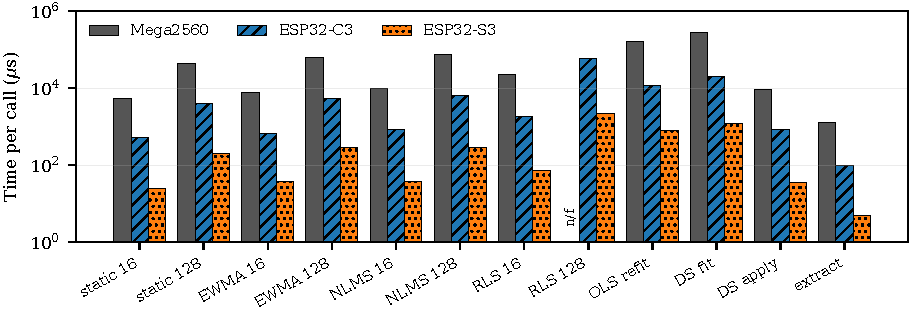
\includegraphics[width=\textwidth]{figures/timing.pdf}
\caption{Measured time per call on the three boards (median, log scale). ``n/f'': RLS at $d=128$ does not fit the Mega2560. Classification and update kernels include feature preprocessing; block OLS and DS fit are executed once per calibration session.}
\label{fig:timing}
\end{figure*}

Three observations follow from these measurements. First, all kernels are fast compared with the measurement cycle of a MOX array, which lasts minutes. The slowest per-sample kernel on the Mega2560, classification with an NLMS update at $d=128$, takes 75~ms. A DS fit from 16 pairs takes 0.27~s in E5, and 0.29~s together with the fusion in E7, and it is executed once per calibration session; after fusion, DS costs no more than the static head. The streaming extractor, which has to keep up with the 100~Hz sampling, occupies 12.7\% of the Mega2560, 1.0\% of the ESP32-C3 and 0.05\% of the ESP32-S3.

Second, label-driven adaptation is cheap compared with inference itself. An NLMS update increases the time of a static classification by a factor of 1.5--1.8 on all boards, and RLS at $d=16$ by a factor of 2.9--4.1. On processors without a floating-point unit, the preprocessing with one logarithm per feature dominates the static classification.

Third, the ESP32-C3, which has no floating-point unit either, is 10.7--14.1 times faster than the Mega2560, close to the ratio of their clock frequencies, and the ESP32-S3 with a single-precision unit is a further 15--27 times faster. Since the instruction set, the memory system and the compiler also differ between the boards, these ratios describe the tested builds and do not isolate the effect of the floating-point unit.

\section{Discussion}
\label{sec:discussion}
The results allow us to draw a deployment map. On an 8-bit microcontroller with 8~kB of SRAM every method with compact features fits, and the choice is decided by the references that can be obtained. Without any labels, EWMA standardisation is a reasonable first step: it costs 132~B and improved the drift stream in most batches and the transfer between boards on average, although it can lose accuracy in single batches and when the gases arrive in long blocks. When a calibration session with about 20 known samples of all gases is possible, RLS or block least squares on 16 features give 0.88--0.90 on the 36-month stream with 1.6--1.7~kB of RAM. Component correction, which reaches 0.658 at $d=128$, is not part of this map, because at a similar RAM budget RLS with compact features is far more accurate. When the instrument is a copy of a calibrated master and 16 pairs covering all gases are available, DS fused into the head gives 0.95 with 272~B of persistent RAM; on cleaned data its advantage over RLS and the simpler paired corrections is small, so that the decisive argument for DS on a small device is its memory. The full-feature variants of RLS, block least squares and DS do not fit the Mega2560 and require an ESP32-class device, where full-feature RLS costs 2.1~ms per sample on the S3 and 58~ms on the C3.

Time, in contrast, does not restrict the choice on any of the boards for the cycle times of MOX arrays. This conclusion is specific to slow chemical sensing; for faster sensors, or for many arrays served by one processor, the measured times can be used directly to estimate the load.

The work has a number of limitations. The accuracy figures of E2 come from one 36-month stream of one instrument, in which the gases are known to be recorded in temporal clusters \cite{dennler}, and E4 rests on five boards; the per-batch spread in Table~\ref{tab:stats} is a better guide to the uncertainty than intervals over seeds, and the board bootstrap gives only a coarse indication. The favourable calibration of E2 and the random transfer pairs of E4 overstate what label-driven updates and DS achieve when a session contains one or two gases, as the post hoc analyses show. The analyses of E6 and E7 were added after the protocol was frozen, and several hyperparameters lie on the edges of their grids. We have not examined label noise or mispaired transfer samples, against which robust losses would have to be tested at the same memory budget. The head is a linear least-squares classifier, weaker than the ensembles and domain-adaptation models used on the same data \cite{vergara,zhang,mida}, and compact nonlinear models such as small random-feature or lookup-table heads were not considered. The planned Q15 versions of the kernels are not included. Finally, each board type was represented by one unit, and energy consumption and worst-case execution time, which matter for battery-powered devices, were not measured.

\section{Conclusion}
In this work we have measured, for MOX electronic noses, the accuracy of linear drift-compensation and calibration-transfer methods together with their RAM and their execution time on three microcontrollers. The results allow the following conclusions.
\begin{enumerate}
\item Without labels, running standardisation of the features improved the static classifier on the 36-month drift stream from 0.498 to 0.614 with 1\,028~B, in seven of eight test batches, and between twin boards from 0.831 to 0.895 with 132~B. Its effect is not uniform, and it decreases when the gases arrive in blocks.
\item With 20 references per batch from all gases, RLS on the classifier reaches 0.923 but keeps 69.7~kB in RAM, while on compact features RLS and block least squares reach 0.876 and 0.898 with 1.6--1.7~kB. In a post hoc analysis with references of a single gas, the benefit of the label-driven updates largely disappears, and several of them fall below the static classifier.
\item Between twin boards, direct standardisation on 16 compact features reaches 0.955 with 16 transfer pairs from all gases; fused into the classifier, it keeps 272~B in RAM and needs 4.6~kB during the fit. With pairs from only one or two gases, it loses its advantage over the static classifier.
\item The float32 kernels reproduce the host on complete streams, also on the three boards, with at most four near-tie differences per 13\,285 predictions for RLS. Even on the Mega2560 the slowest per-sample kernel takes 75~ms, so that for gas sensor arrays it is memory rather than time that limits the choice of method.
\end{enumerate}
These conclusions rest on one drift dataset and five twin boards, and their confirmation with a physical sensor array and realistic calibration sessions, together with fixed-point kernels and energy measurements, is the next step of our work.

\section*{Data and Code Availability}
The protocol, source code, results, firmware sources, raw board logs and the log of post hoc changes are available in the public repository \cite{code}, which will be archived with a DOI on acceptance. The E1/E2 protocol was frozen at commit \texttt{4a439fb} and E3/E4 at \texttt{c9799aa}; the E5 firmware is at \texttt{578719c}, and its board captures and their analysis at \texttt{4e8adc1}. The E7 captures are in \texttt{results/e7\_20261110}; the commit of each run is identified there by the SHA-256 digests of its sources. The datasets are available from the UCI repository \cite{uci224,uci270,uci361} and are not redistributed.

\section*{Acknowledgment}
The author used Anthropic Claude to assist in writing the analysis and firmware code and in drafting and editing the manuscript. The author reviewed and verified all code, results and text and takes full responsibility for the content.

\begin{thebibliography}{99}
\bibitem{persaud} K. C. Persaud and G. H. Dodd, ``Analysis of discrimination mechanisms in the mammalian olfactory system using a model nose,'' \emph{Nature}, vol. 299, no. 5881, pp. 352--355, 1982, doi: \href{https://doi.org/10.1038/299352a0}{10.1038/299352a0}.
\bibitem{marco} S. Marco and A. Guti\'errez-G\'alvez, ``Signal and data processing for machine olfaction and chemical sensing: A review,'' \emph{IEEE Sensors J.}, vol. 12, no. 11, pp. 3189--3214, Nov. 2012.
\bibitem{artursson} T. Artursson, T. Ekl\"ov, I. Lundstr\"om, P. M\aa rtensson, M. Sj\"ostr\"om, and M. Holmberg, ``Drift correction for gas sensors using multivariate methods,'' \emph{J. Chemometrics}, vol. 14, nos. 5--6, pp. 711--723, 2000.
\bibitem{padilla} M. Padilla, A. Perera, I. Montoliu, A. Chaudry, K. Persaud, and S. Marco, ``Drift compensation of gas sensor array data by orthogonal signal correction,'' \emph{Chemometr. Intell. Lab. Syst.}, vol. 100, no. 1, pp. 28--35, 2010, doi: \href{https://doi.org/10.1016/j.chemolab.2009.10.002}{10.1016/j.chemolab.2009.10.002}.
\bibitem{ziyatdinov} A. Ziyatdinov, S. Marco, A. Chaudry, K. Persaud, P. Caminal, and A. Perera, ``Drift compensation of gas sensor array data by common principal component analysis,'' \emph{Sens. Actuators B, Chem.}, vol. 146, no. 2, pp. 460--465, 2010, doi: \href{https://doi.org/10.1016/j.snb.2009.11.034}{10.1016/j.snb.2009.11.034}.
\bibitem{vergara} A. Vergara, S. Vembu, T. Ayhan, M. A. Ryan, M. L. Homer, and R. Huerta, ``Chemical gas sensor drift compensation using classifier ensembles,'' \emph{Sens. Actuators B, Chem.}, vols. 166--167, pp. 320--329, 2012, doi: \href{https://doi.org/10.1016/j.snb.2012.01.074}{10.1016/j.snb.2012.01.074}.
\bibitem{zhang} L. Zhang and D. Zhang, ``Domain adaptation extreme learning machines for drift compensation in E-nose systems,'' \emph{IEEE Trans. Instrum. Meas.}, vol. 64, no. 7, pp. 1790--1801, Jul. 2015.
\bibitem{rodriguez} I. Rodriguez-Lujan, J. Fonollosa, A. Vergara, M. Homer, and R. Huerta, ``On the calibration of sensor arrays for pattern recognition using the minimal number of experiments,'' \emph{Chemometr. Intell. Lab. Syst.}, vol. 130, pp. 123--134, 2014, doi: \href{https://doi.org/10.1016/j.chemolab.2013.10.012}{10.1016/j.chemolab.2013.10.012}.
\bibitem{wang} Y. Wang, D. J. Veltkamp, and B. R. Kowalski, ``Multivariate instrument standardization,'' \emph{Anal. Chem.}, vol. 63, no. 23, pp. 2750--2756, 1991, doi: \href{https://doi.org/10.1021/ac00023a016}{10.1021/ac00023a016}.
\bibitem{fonollosa} J. Fonollosa, L. Fern\'andez, A. Guti\'errez-G\'alvez, R. Huerta, and S. Marco, ``Calibration transfer and drift counteraction in chemical sensor arrays using direct standardization,'' \emph{Sens. Actuators B, Chem.}, vol. 236, pp. 1044--1053, 2016, doi: \href{https://doi.org/10.1016/j.snb.2016.05.089}{10.1016/j.snb.2016.05.089}.
\bibitem{li2026} R. Li, Z. Li, B. A. Kofi, J. Sun, Y. He, and M. Jiao, ``A comprehensive review of algorithms for drift compensation in metal oxide semiconductor gas sensor arrays,'' \emph{Chemosensors}, vol. 14, no. 6, Art. no. 143, 2026, doi: \href{https://doi.org/10.3390/chemosensors14060143}{10.3390/chemosensors14060143}.
\bibitem{krayden} A. Krayden, M. Avraham, H. Ashkar, T. Blank, S. Stolyarova, and Y. Nemirovsky, ``TinyML-based real-time drift compensation for gas sensors using spectral--temporal neural networks,'' \emph{Chemosensors}, vol. 13, no. 7, Art. no. 223, 2025, doi: \href{https://doi.org/10.3390/chemosensors13070223}{10.3390/chemosensors13070223}.
\bibitem{liu2019} T. Liu \emph{et al.}, ``Active learning on dynamic clustering for drift compensation in an electronic nose system,'' \emph{Sensors}, vol. 19, no. 16, Art. no. 3601, 2019, doi: \href{https://doi.org/10.3390/s19163601}{10.3390/s19163601}.
\bibitem{cao2021} J. Cao, T. Liu, J. Chen, T. Yang, X. Zhu, and H. Wang, ``Drift compensation on massive online electronic-nose responses,'' \emph{Chemosensors}, vol. 9, no. 4, Art. no. 78, 2021, doi: \href{https://doi.org/10.3390/chemosensors9040078}{10.3390/chemosensors9040078}.
\bibitem{sun2022} F. Sun, R. Sun, and J. Yan, ``Cross-domain active learning for electronic nose drift compensation,'' \emph{Micromachines}, vol. 13, no. 8, Art. no. 1260, 2022, doi: \href{https://doi.org/10.3390/mi13081260}{10.3390/mi13081260}.
\bibitem{tinytrain} J. Lin, L. Zhu, W.-M. Chen, W.-C. Wang, C. Gan, and S. Han, ``On-device training under 256KB memory,'' in \emph{Adv. Neural Inf. Process. Syst.}, 2022. [Online]. Available: \url{https://arxiv.org/abs/2206.15472}
\bibitem{uci224} A. Vergara, ``Gas sensor array drift dataset,'' UCI Machine Learning Repository, 2012. [Online]. Available: \url{https://archive.ics.uci.edu/dataset/224}
\bibitem{uci270} A. Vergara, ``Gas sensor array drift dataset at different concentrations,'' UCI Machine Learning Repository, 2013. [Online]. Available: \url{https://archive.ics.uci.edu/dataset/270}
\bibitem{muezzinoglu} M. K. Muezzinoglu, A. Vergara, R. Huerta, N. Rulkov, M. I. Rabinovich, A. Selverston, and H. D. I. Abarbanel, ``Acceleration of chemo-sensory information processing using transient features,'' \emph{Sens. Actuators B, Chem.}, vol. 137, no. 2, pp. 507--512, 2009, doi: \href{https://doi.org/10.1016/j.snb.2008.10.065}{10.1016/j.snb.2008.10.065}.
\bibitem{uci361} J. Fonollosa, ``Twin gas sensor arrays,'' UCI Machine Learning Repository, 2016, doi: \href{https://doi.org/10.24432/C5MW3K}{10.24432/C5MW3K}.
\bibitem{haykin} S. Haykin, \emph{Adaptive Filter Theory}, 5th ed. Upper Saddle River, NJ, USA: Pearson, 2014.
\bibitem{davison} A. C. Davison and D. V. Hinkley, \emph{Bootstrap Methods and Their Application}. Cambridge, U.K.: Cambridge Univ. Press, 1997.
\bibitem{code} O. Kuznetsov, ``enose-drift-mcu: Drift compensation and calibration transfer for electronic noses on microcontrollers,'' GitHub, 2026. [Online]. Available: \url{https://github.com/KuznetsovKarazin/enose-drift-mcu}
\end{thebibliography}

\end{document}
